\documentclass[11pt]{article}
\usepackage{amssymb}
\usepackage{amsfonts}
\usepackage{amsmath}
\usepackage{bm}
\usepackage{latexsym}
\usepackage{epsfig}

\usepackage{tikz}
\usetikzlibrary{arrows,decorations.pathmorphing,backgrounds,positioning,fit,petri}

\setlength{\evensidemargin}{.25in}
\setlength{\textwidth}{6in}
\setlength{\topmargin}{-0.4in}
\setlength{\textheight}{8.5in}


\newcommand{\handout}[5]{
   \renewcommand{\thepage}{#1-\arabic{page}}
   \noindent
   \begin{center}
   \framebox{
      \vbox{
    \hbox to 5.78in {{\sf 18.312: Algebraic Combinatorics} 
\hfill \sf #2 }
       \vspace{4mm}
       \hbox to 5.78in { {\Large \hfill #5  \hfill} }
       \vspace{2mm}
       \hbox to 5.78in { {\em #3 \hfill #4} }
      }
   }
   \end{center}
   \vspace*{4mm}
}

\newcommand{\lecture}[4]{\handout{#1}{#2}{Lecture date: #3}{Notes by: #4}{Lecture #1}}


\textwidth=6in
\oddsidemargin=0.25in
\evensidemargin=0.25in
\topmargin=-0.1in
\footskip=0.8in
\parindent=0.0cm
\parskip=0.3cm
\textheight=8.00in
\setcounter{tocdepth} {3}
\setcounter{secnumdepth} {2}
\sloppy

\newtheorem{theorem}{Theorem}
\newtheorem{lemma}[theorem]{Lemma}
\newtheorem{proposition}[theorem]{Proposition}
\newtheorem{corollary}[theorem]{Corollary}
\newtheorem{fact}[theorem]{Fact}
\newtheorem{definition}[theorem]{Definition}
\newtheorem{remark}[theorem]{Remark}
\newtheorem{conjecture}[theorem]{Conjecture}
\newtheorem{question}[theorem]{Question}
\newtheorem{answer}[theorem]{Answer}
\newtheorem{exercise}[theorem]{Exercise}
\newtheorem{example}[theorem]{Example}
\newenvironment{proof}{\noindent \textbf{Proof:}}{$\Box$}

\newcommand{\N}{\mathbb N} % natural numbers 0,1,2,...
\newcommand{\Z}{\mathbb Z}  % integers
\newcommand{\R}{\mathbb R} % reals
\newcommand{\C}{\mathbb C} % complex numbers
\newcommand{\F}{\mathbb F} % finite fields

\newcommand{\floor}[1]{\left\lfloor {#1} \right\rfloor} % floor function
\newcommand{\ceiling}[1]{\left\lceil {#1} \right\rceil} % ceiling function
\newcommand{\binomial}[2]{\left( \begin{array}{c} {#1} \\ 
                        {#2} \end{array} \right)} % binomial coefficients
\newcommand{\modulo}[1]{\quad (\mbox{mod }{#1})} %congruences

\newcommand{\ignore}[1]{} % useful for commenting things out



\begin{document}
\lecture{19}{Lionel Levine}{April 21, 2011}{David Witmer} 
% replace n in the line above (and in the file name) by an actual integer
% replace Feb 1 by the date of the lecture 

\section{Matrix-Tree Theorem}

\subsection{Undirected Graphs}

Let $G = (V,E)$ be a connected, undirected graph with $n$ vertices, and let $\kappa(G)$ be the number of spanning trees of $G$.

\begin{definition}[Laplacian matrix of undirected graph]
The Laplacian matrix $L$ of $G$ is equal to $D - A$, where
$$
D = \begin{pmatrix}
d_1 & & 0 \\
& \ddots & \\
0 & & d_n
\end{pmatrix}
$$
such that $d_i$ is the degree of vertex $i$, i.e. the number of edges incident to vertex $i$, and $A$ is the adjacency matrix of $G$ such that
$$ A = (a_{ij}),$$
$$a_{ij} =
\begin{cases}
1 ~~\mathrm{if}~(i,j) \in E \\
0 ~~\mathrm{else.}
\end{cases}
$$
\end{definition}

\begin{theorem}[Matrix-Tree Theorem, Version 1]
$$\kappa(G) = \frac{1}{n}\lambda_1\lambda_2\ldots\lambda_{n-1},$$
where $\lambda_1$, $\lambda_2$, $\ldots$, $\lambda_{n-1}$ are non-zero eigenvalues of the Laplacian matrix $L$ of $G$.
\end{theorem}

\subsection{Directed Graphs}

We can give another version of the Matrix-Tree Theorem for directed graphs.  First, we need to define spanning trees and Laplacian matrices for directed graphs.  Let $\Gamma = (V,E)$ be a directed graph.

\begin{definition}[Oriented spanning tree]
An oriented spanning tree of $\Gamma$ rooted at $r \in V$ is a spanning subgraph $T = (V,A)$ such that
\begin{enumerate}
\item Every vertex $v \neq r$ has out degree 1.
\item $r$ has out degree 0.
\item $T$ has no oriented cycles.
\end{enumerate}
\end{definition}

\begin{example}
Consider the following directed graph:
\begin{center}
\begin{tikzpicture}
	\path (0,0) node (1) [shape=circle,draw, inner sep=2pt] [label=left:1] {}
		  (0,-1) node (2) [shape=circle,draw, inner sep=2pt] [label=left:2] {}
		  (1,-1) node (3) [shape=circle,draw, inner sep=2pt] [label=right:3] {}
		  (1,0) node (4) [shape=circle,draw, inner sep=2pt] [label=right:\text{r=4}] {};
	\draw[->] (1) -- (4);
	\draw[->] (2) -- (1);
	\draw[->] (3) -- (2);
	\draw[->] (4) -- (3);
	\draw[->] (1) -- (3);
	\draw[->] (3) to [out=65,in=305] (4);
\end{tikzpicture}
\end{center}

It has three oriented spanning trees:
\begin{center}
\begin{tikzpicture}
	\path (0,0) node (1) [shape=circle,draw, inner sep=2pt] [label=left:1] {}
		  (0,-1) node (2) [shape=circle,draw, inner sep=2pt] [label=left:2] {}
		  (1,-1) node (3) [shape=circle,draw, inner sep=2pt] [label=right:3] {}
		  (1,0) node (4) [shape=circle,draw, inner sep=2pt] [label=right:\text{r=4}] {};
	\draw[->] (1) -- (4);
	\draw[->] (2) -- (1);
	\draw[->] (3) -- (2);
\end{tikzpicture}

\begin{tikzpicture}
	\path (0,0) node (1) [shape=circle,draw, inner sep=2pt] [label=left:1] {}
		  (0,-1) node (2) [shape=circle,draw, inner sep=2pt] [label=left:2] {}
		  (1,-1) node (3) [shape=circle,draw, inner sep=2pt] [label=right:3] {}
		  (1,0) node (4) [shape=circle,draw, inner sep=2pt] [label=right:\text{r=4}] {};
	\draw[->] (2) -- (1);
	\draw[->] (1) -- (3);
	\draw[->] (3) -- (4);
\end{tikzpicture}

\begin{tikzpicture}
	\path (0,0) node (1) [shape=circle,draw, inner sep=2pt] [label=left:1] {}
		  (0,-1) node (2) [shape=circle,draw, inner sep=2pt] [label=left:2] {}
		  (1,-1) node (3) [shape=circle,draw, inner sep=2pt] [label=right:3] {}
		  (1,0) node (4) [shape=circle,draw, inner sep=2pt] [label=right:\text{r=4}] {};
	\draw[->] (2) -- (1);
	\draw[->] (1) -- (4);
	\draw[->] (3) -- (4);
\end{tikzpicture}

\end{center}
\end{example}

\begin{definition}[Laplacian matrix of directed graph]
The Laplacian matrix $L$ of $\Gamma$ is equal to $D - A$, where
$$
D = \begin{pmatrix}
d_1 & & 0 \\
& \ddots & \\
0 & & d_n
\end{pmatrix}
$$
such that $d_i$ is the out degree of vertex $i$, i.e. $\#\{j \in V | (i,j) \in E\}$, and $A$ is the adjacency matrix of $\Gamma$.
\end{definition}

\begin{theorem}[Matrix-Tree Theorem, Version 2]
Let $$\kappa(\Gamma,r) = \#\{\textup{oriented spanning trees of $\Gamma$ rooted at $r$}\}$$ and $L_r$ be the Laplacian matrix of $\Gamma$ with the row and column corresponding to vertex $r$ crossed out.  Then
$$\kappa(\Gamma,r) = \det{L_r}$$
where $L_r$ is the Laplacian matrix $L$ with row and column $r$ removed.
\end{theorem}

\begin{example}
Consider the directed graph from the previous example:
\begin{center}
\begin{tikzpicture}
	\path (0,0) node (1) [shape=circle,draw, inner sep=2pt] [label=left:1] {}
		  (0,-1) node (2) [shape=circle,draw, inner sep=2pt] [label=left:2] {}
		  (1,-1) node (3) [shape=circle,draw, inner sep=2pt] [label=right:3] {}
		  (1,0) node (4) [shape=circle,draw, inner sep=2pt] [label=right:\text{r=4}] {};
	\draw[->] (1) -- (4);
	\draw[->] (2) -- (1);
	\draw[->] (3) -- (2);
	\draw[->] (4) -- (3);
	\draw[->] (1) -- (3);
	\draw[->] (3) to [out=65,in=305] (4);
\end{tikzpicture}
\end{center}
Then we see that
$$
D = \begin{pmatrix}
2 & 0 & 0 & 0 \\
0 & 1 & 0 & 0 \\
0 & 0 & 2 & 0 \\
0 & 0 & 0 & 1
\end{pmatrix}
$$
and
$$
A = \begin{pmatrix}
0 & 1 & 0 & 0 \\
0 & 0 & 1 & 0 \\
1 & 0 & 0 & 1 \\
1 & 0 & 1 & 0
\end{pmatrix}
$$
so
$$
L = \begin{pmatrix}
2 & -1 & 0 & 0 \\
0 & 1 & -1 & 0 \\
-1 & 0 & 2 & -1 \\
-1 & 0 & -1 & 1
\end{pmatrix}
$$
and
$$
L_r = \begin{pmatrix}
2 & -1 & 0 \\
0 & 1 & -1 \\
-1 & 0 & 2 \\
\end{pmatrix}
$$
Then
$$ \det{L_r} = 2 \cdot 1 \cdot 2 + -1 \cdot -1 \cdot -1 = 3$$
which matches what we found in the previous example.
\end{example}

We will prove this version of the Matrix-Tree Theorem and then show that it implies the version for undirected graphs.

\begin{proof}
Reorder the vertices of $\Gamma$ so that $r$ is the $n$th vertex. 
Then $\det{L_r} = d_1 d_2 \ldots d_{n-1} - (\textup{other terms})$, since $L_r$ has the $d_i$'s on the diagonal and either $-1$ or $0$ for the off-diagonal entries.  $d_1 d_2 \ldots d_{n-1}$ counts the number of subgraphs $H$ of $\Gamma$ such that each vertex $v \neq r$ has out-degree 1.  So we have that
$$H = T \cup C_1 \cup \cdots \cup C_k,$$
where $T$ is an oriented tree rooted at $r$ and each $C_i$ is an oriented cycle.

 Then
$$\det{L_r} = \sum_{\sigma \in S_{n-1}}{\mathrm{sgn}{(\sigma)} L_{1, \sigma(1)} \ldots L_{n-1, \sigma(n-1)}}.$$
Let $\mathrm{fix}{(\sigma)} = \{i~|~\sigma(i) = i\}$.  Then we have
$$\det{L_r} = \sum_{\sigma \in S_{n-1}}{\mathrm{sgn}{(\sigma)} \prod_{i \in \mathrm{fix}{(\sigma)}}{d_i} \prod_{i \notin \mathrm{fix}{(\sigma)}} L_{i, \sigma(i)}}.$$
$\prod_{i \notin \mathrm{fix}{(\sigma)}} L_{i, \sigma(i)}$ is only non-zero when $(i,\sigma(i)) \in E$ for all $i \notin \mathrm{fix}{(\sigma)}$.  In this case,
$$\prod_{i \notin \mathrm{fix}{(\sigma)}} L_{i, \sigma(i)} = (-1)^{n-1-|\mathrm{fix}(\sigma)|} .$$

We wish to write
$$ \det{L_r} = \sum_{\textup{subgraphs $H \subset \Gamma$}}{C_H},$$
where $C_H$ is 1 if $H$ is an oriented spanning tree and 0 otherwise.  Any permutation $\sigma$ consists of fixed points and cycles.  A subgraph $H = T \cup C_1 \cup \cdots \cup C_k$ arises from $\sigma$ if and only if the union of all cycles $C_i$ of $H$ contains all vertices not fixed by $H$, which, in turn, is true if and only if $T \subseteq \mathrm{fix}(\sigma)$.

We can then conclude that
$$C_H = \sum_{\{\sigma \in S_{n-1}~|~T \subseteq \mathrm{fix}(\sigma)\}} \mathrm{sgn}(\sigma) (-1)^{n-1-|\mathrm{fix}(\sigma)|}.$$
Our goal is then to show that $C_H$ is 1 when $H$ is a tree and 0 otherwise.  When $H$ is a tree, $H = T$ and there are no cycles.  Then all vertices are in $|\mathrm{fix}(\sigma)|$ and $\sigma$ is the identity permutation.  The sign of the identity permutation is 1 and $n-1$ points are fixed, so $C_H = 1$.

Lastly, we need to show that $C_H = 0$ if $k \geq 1$, i.e. if $H$ has a cycle.  For each $C_i$, we can either choose $C_i \subset \mathrm{fix}(\sigma)$ or $C_i$ to be a cycle of $\sigma$.  Let $i_1, \ldots, i_l$ be the indices of the $C_i$'s that are formed from vertices in cycles of $\sigma$.  All other points must be fixed by $\sigma$, so
$$\mathrm{sgn}(\sigma) = (-1)^{(|C_{i_1}|-1) + \ldots + (|C_{i_l}|-1)}.$$
This means that
$$C_H = \sum_{\{i_1, \ldots, i_l\} \in [k]} (-1)^{(|C_{i_1}|-1) + \ldots + (|C_{i_l}|-1)} (-1)^{|C_{i_1}|+\ldots+|C_{i_l}|}.$$
So,
$$
\begin{aligned}
C_H &= \sum_{S \subseteq [k]} (-1)^{|S|} \\
&= \sum_{l=0}^k \binom{k}{l} (1-1)^k \\
&= 0~\textup{if $k \geq 1$}.
\end{aligned}
$$
\end{proof}

\subsection{Proof of the Matrix Tree Theorem, Version 1}

Now we will show that Version 2 of the Matrix Tree Theorem implies the version for undirected graphs.

\begin{proof}
Given undirected graph $G$, let $\Gamma$ be the directed graph with edges $(i,j)$ and $(j,i)$ for every edge of $G$.  We first observe that there is a bijection between the set of oriented spanning trees of $\Gamma$ rooted at $r$ and the set of spanning trees of $G$.  We can take any oriented spanning tree of $\Gamma$ rooted at $r$ and get a spanning tree of $G$ by disregarding the root and the orientation of the edges.  For any spanning tree $T$ of $G$, we can get an oriented spanning tree of $\Gamma$ by orienting edges along the unique path from each vertex to $r$.  Such a path exists because $T$ is connected and is unique because $T$ has no cycles.  Then

$$n\kappa(G) = \sum_{r=1}^n \kappa(\Gamma,r).$$

Let $L$ be the Laplacian matrix of $\Gamma$.  Then the characteristic polynomial of $L$ is
$$\chi(t) = \det{(tI - L)}.$$
It is true that
$$\sum_{r=1}^n \det{L_r} = (-1)^{n-1} [t] \chi(t),$$
where $[t] \chi(t)$ is the coefficient of $t$ in $\chi(t)$.

So, we have that
$$
\begin{aligned}
n \kappa(G) = \sum_{r-1}^n \det{L_r} &= (-1)^{n-1} [t] \chi(t) \\
&= (-1)^{n-1} [t] \prod_{i=1}^n(t-\lambda_i), \textup{  where the $\lambda_i$'s are eigenvalues of $L$ and $\lambda_n=0$} \\
&= (-1)^{n-1} (-1)^{n-1} \lambda_1 \ldots \lambda_{n-1} \\
&= \lambda_1 \ldots \lambda_{n-1}.
\end{aligned}
$$
Therefore,
$$ \kappa(G) = \frac{1}{n} \lambda_1 \ldots \lambda_{n-1}.$$
\end{proof}

\section{Cayley's Theorem}

\begin{theorem}[Cayley's Theorem]
The number of trees on $n$ labeled vertices is $n^{n-2}$.
\end{theorem}

\begin{example}
Consider trees containing 4 vertices.  There are $16 = 4^{4-2}$ total, 4 of the form

\begin{center}
\begin{tikzpicture}
	\path (0,0) node (1) [shape=circle,draw, inner sep=2pt] [label=above:1] {}
		  (0,-1) node (2) [shape=circle,draw, inner sep=2pt] [label=below:2] {}
		  (-1,-1) node (3) [shape=circle,draw, inner sep=2pt] [label=below:3] {}
		  (1,-1) node (4) [shape=circle,draw, inner sep=2pt] [label=below:4] {};
	\draw (1) -- (2);
	\draw (1) -- (3);
	\draw (1) -- (4);
\end{tikzpicture}
\end{center}

and 12 of the form

\begin{center}
\begin{tikzpicture}
	\path (0,0) node (1) [shape=circle,draw, inner sep=2pt] [label=below:1] {}
		  (1,0) node (2) [shape=circle,draw, inner sep=2pt] [label=below:2] {}
		  (2,0) node (3) [shape=circle,draw, inner sep=2pt] [label=below:3] {}
		  (3,0) node (4) [shape=circle,draw, inner sep=2pt] [label=below:4] {};
	\draw (1) -- (2);
	\draw (2) -- (3);
	\draw (3) -- (4);
\end{tikzpicture}
\end{center}
\end{example}

\begin{proof}
Any tree on $n$ vertices is a spanning tree of the complete graph $K_n$, so we can apply Version 2 of the Matrix-Tree Theorem.
So,
$$\kappa(K_n) = \frac{1}{n} \lambda_1 \ldots \lambda_{n-1},$$
where $$\lambda_1, \ldots, \lambda_{n-1}$$ are the non-zero eigenvalues of the Laplacian matrix
$$L = 
\begin{pmatrix}
n-1 & -1 & \cdots & -1 \\
-1 & n-1 & \cdots & -1 \\
\vdots & \vdots & \ddots & \vdots \\
-1 & -1 & \cdots & n-1
\end{pmatrix}
= nI - J,
$$
where $J$ is the $n \times n$ matrix of ones.

$J$ has the ones vector as one of its eigenvectors.  The remaining $n-1$ eigenvectors are of the form
$$
\begin{pmatrix}
\vdots\\
1 \\
-1 \\
\vdots
\end{pmatrix},
$$
so $J$ has eigenvalues $n, 0, \ldots, 0$, with 0 having multiplicity $n-1$.  This implies that $L$ has eigenvalues $0,n,\ldots,n$, with $n$ having multiplicity $n-1$.

So,
$$\kappa(K_n) = \frac{n^{n-1}}{n} = n^{n-2}.$$
\end{proof}

\section{Eigenvalues of the Adjacency Matrix}

Let $G$ be an undirected, connected graph with $n$ vertices.  Let $P_l$ be the number of closed paths in $G$ of length $l$:
$$P_l = \#\{(v_0,v_1,\ldots,v_{l-1},v_l = v_0)~|~(v_i,v_{i+1}) \in E \textup{ for $i = 0,1,\ldots,l-1$}\}$$

\begin{theorem}
$$P_l = \phi_1^l + \cdots + \phi_n^l,$$
where $\phi_1, \ldots, \phi_n$ are the eigenvalues of the adjacency matrix $A$ of $G$.
\end{theorem}

\begin{proof}
We observe that
$$ (A^l)_{ij} = \#\{\text{paths of length $l$ from $i$ to $j$}\}.$$

So,
$$P_l = (A^l)_{11} + (A^l)_{22} + \cdots + (A^l)_{nn} = \mathrm{Tr}(A^l).$$
Note that this holds for both directed and undirected graphs.

Since $G$ is undirected, $A$ is symmetric, which means that $A$ is diagonalizable so there exists some $S$ such that
$$ SAS^{-1} = 
\begin{pmatrix}
\phi_1 & 0 & \cdots & 0 \\
0 & \phi_2 & \cdots & 0 \\
\vdots & \vdots & \ddots & \vdots \\
0 & 0 & \cdots & \phi_n
\end{pmatrix}.
$$

So,
$$
\begin{aligned}
P_l &= \mathrm{Tr}(A^l) \\
&= \mathrm{Tr}(SA^lS^{-1}) \\
&= \mathrm{Tr}((SAS^{-1})^l) \\
&= \mathrm{Tr}
\begin{pmatrix}
\phi_1^l & 0 & \cdots & 0 \\
0 & \phi_2^l & \cdots & 0 \\
\vdots & \vdots & \ddots & \vdots \\
0 & 0 & \cdots & \phi_n^l
\end{pmatrix}\\
&= \phi_1^l + \cdots + \phi_n^l.
\end{aligned}
$$
\end{proof}

\end{document}
